\documentclass[12pt]{article}
\usepackage{auck2e,multicol,amssymb,amsmath,color}
\usepackage{epsfig}
\usepackage[english]{babel}
\usepackage{blindtext}
\usepackage{microtype}
\usepackage{minted}

%\usepackage{graphicx}
\newcommand{\ds}{\displaystyle}
\newcommand{\mmark}[1]{[{#1 mark(s)}]}
\newcommand{\markk}[1]{[{\bf #1 marks}]}
\newcommand{\dspace}{\renewcommand{\baselinestretch}{2} \small \normalsize}
\newcommand{\sspace}{\renewcommand{\baselinestretch}{1} \small \normalsize}
\newcommand{\btheta}{\mbox{\boldmath $\theta$}}
\newcommand{\blambda}{\mbox{\boldmath $\lambda$}}
\newcommand{\bTheta}{\mbox{\boldmath $\Theta$}}
\newcommand{\bzeta}{\mbox{\boldmath $\zeta$}}
\newcommand{\bpi}{\mbox{\boldmath $\pi$}}
\newcommand{\bphi}{\mbox{\boldmath $\phi$}}
\newcommand{\ba}{\mbox{\boldmath $a$}}
\newcommand{\bb}{\mbox{\boldmath $b$}}
\newcommand{\bd}{\mbox{\boldmath $d$}}
\newcommand{\bm}{\mbox{\boldmath $m$}}
\newcommand{\bx}{\mbox{\boldmath $x$}}
\newcommand{\bh}{\mbox{\boldmath $h$}}
\newcommand{\bu}{\mbox{\boldmath $u$}}
\newcommand{\bP}{\mbox{\boldmath $P$}}
\newcommand{\bQ}{\mbox{\boldmath $Q$}}
\newcommand{\bR}{\mbox{\boldmath $R$}}
\newcommand{\by}{\mbox{\boldmath $y$}}
\newcommand{\bY}{\mbox{\boldmath $Y$}}
\newcommand{\bX}{\mbox{\boldmath $X$}}
\newcommand{\bU}{\mbox{\boldmath $U$}}
\newcommand{\bD}{\mbox{\boldmath $D$}}
\newcommand{\bV}{\mbox{\boldmath $V$}}
\newcommand{\bH}{\mbox{\boldmath $H$}}
\newcommand{\bgamma}{\mbox{\boldmath $\gamma$}}
\newcommand{\bGamma}{\mbox{\boldmath $\Gamma$}}
\newcommand{\balpha}{\mbox{\boldmath $\alpha$}}
\newcommand{\bbeta}{\mbox{\boldmath $\beta$}}
\newcommand{\bdelta}{\mbox{\boldmath $\delta$}}
\newcommand{\bomega}{\mbox{\boldmath $\omega$}}
\newcommand{\bpsi}{\mbox{\boldmath $\psi$}}
\newcommand{\bepsilon}{\mbox{\boldmath $\epsilon$}}
\newcommand{\be}{\begin{eqnarray}}
\newcommand{\ee}{\end{eqnarray}}
\def\BackgroundEPS#1#2#3#4{%
    \special{ps: @beginspecial @setspecial initmatrix
                0.9 setgray #2 #3 translate #4 dup scale}
    \special{ps: plotfile #1}
    \special{ps: @endspecial}
}
\newcommand{\wbugs}{{\sffamily\textbf{WinBUGS }}}
\newcommand{\coda}{{\sffamily\textbf{CODA }}}
\newcommand{\glm}{{\sffamily\textbf{G.L.M }}}
\newcommand{\rwb}{{\sffamily\textbf{R2WinBUGS }}}
\newcommand{\rar}{{\sffamily\textbf{Rock and roll man! }}}
\newcommand{\anova}{{\sffamily\textbf{ANOVA }}}
\newcommand{\mcmc}{{\sffamily\textbf{MCMC }}}
\newcommand{\dic}{{\sffamily\textbf{DIC }}}
\newcommand{\dagr}{{\sffamily\textbf{DAG }}}
\newcommand{\boxeq}[1]{%
\fboxrule=0.5mm%
\fboxsep=5mm%
\begin{center}\fcolorbox{black}{yellow}{\begin{minipage}{0.9\linewidth}
\begin{Beqnarray} #1 \end{Beqnarray}\end{minipage}}\end{center}%
\fboxrule=1pt%
\fboxsep=3pt%
}

\newcommand{\boxst}[1]{%
\fboxrule=0.5mm%
\fboxsep=5mm%
\begin{center}\fcolorbox{black}{yellow}{ \begin{minipage}{0.9\linewidth}#1 \end{minipage} }\end{center}%
\fboxrule=1pt%
\fboxsep=3pt%
}
%%%%%%%%%%%%%%%%%%%%%%%%%%%%%%%%%%%%%%%%%%%%%%%%%%%%%%%%%%%%%%%%%%%%%%%%
% Macro         :   \BackgroundEPS{filename}{tx}{ty}{s}
%-----------------------------------------------------------------------
% Description   :   Display an EPS file in the background of the
%                   current page.
%-----------------------------------------------------------------------
% Author        :   Bernard Desruisseaux (bernard@XYZZYcs.mcgill.ca)
%-----------------------------------------------------------------------
% Usage         :   \BackgroundEPS{pic.eps}{80}{100}{2}
%                   \BackgroundEPS{"`gunzip -c pic.eps.gz"}{80}{100}{2}
%                   \BackgroundEPS{"`zcat pic.eps.Z"}{80}{100}{2}
%%%%%%%%%%%%%%%%%%%%%%%%%%%%%%%%%%%%%%%%%%%%%%%%%%%%%%%%%%%%%%%%%%%%%%%%

\newcommand{\given}{\,|\,}

\paper{Introduction to Bayesian Statistics}
\due{Not for assessment}
\thetitle{\textbf{Tutorial 2}} 
\begin{document}


%\BackgroundEPS{bayes.eps}{0}{0}{1.2}
\makeband


\begin{Questions}

\item 
The following histogram shows the `inter-arrival times'
$t_1, t_2, ..., t_N$
of births
over a 24 hour period at a major Brisbane
hospital\footnote{Real data!}. According to theory, the
distribution of these times (the gap between one birth and the next)
should follow an exponential distribution. The number of data points is
$N=43$ and the average of the data (the `sample mean') is
$\bar{t} = \frac{1}{N}\sum_{i=1}^N t_i = 0.554$ hours.

\begin{figure}[!ht]
\centering
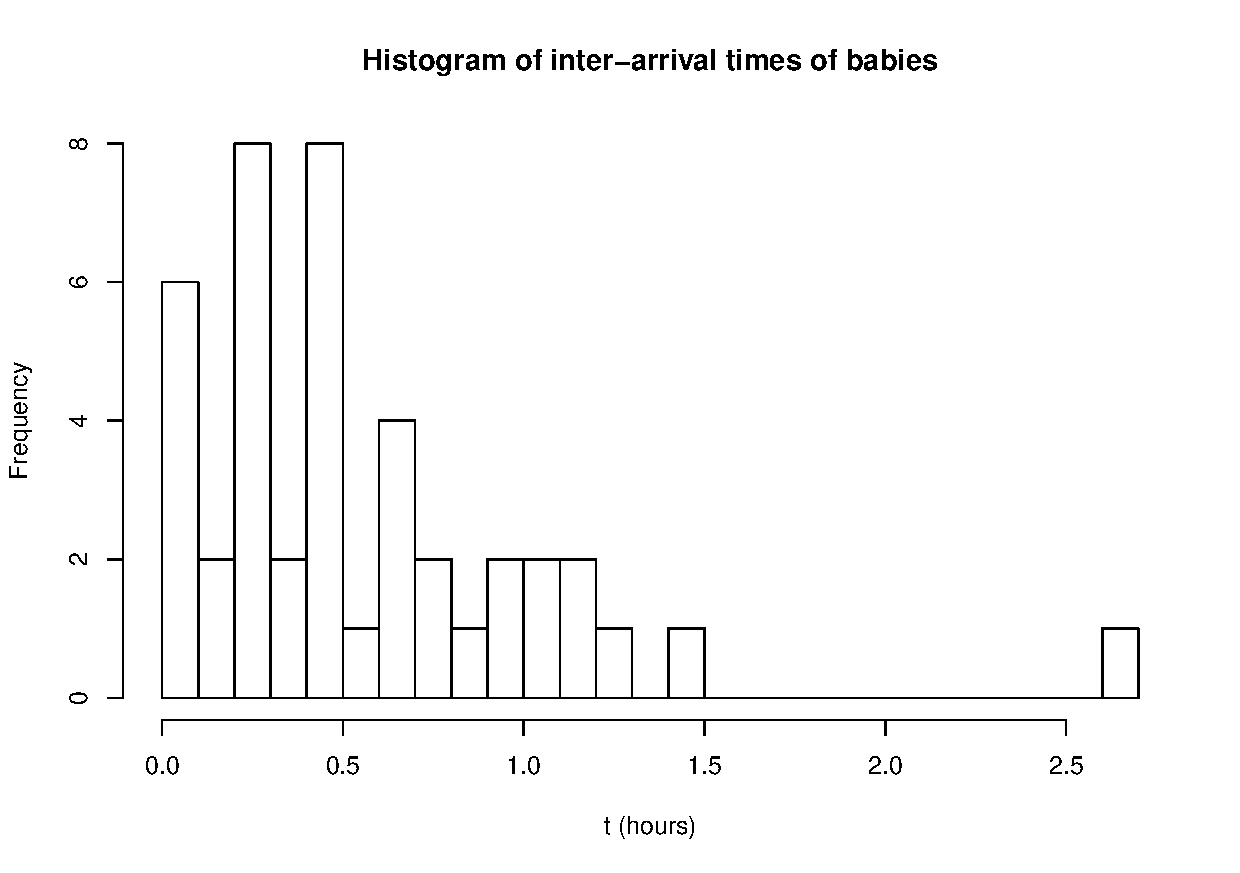
\includegraphics[scale=0.6]{babies.pdf}
\end{figure}

For a single variable $t$, an exponential probability density function is
\begin{align}
p(t | \lambda) &= \lambda e^{-\lambda t}
\end{align}
where $t > 0$ and $\lambda$ is a parameter which controls the width of the
exponential distribution. In fact, the expected value of $t$ is
$1/\lambda$, so $\lambda$ is the expected arrival rate of babies.
In this question you'll `fit an exponential distribution to the data', i.e.,
find the posterior distribution for $\lambda$ given the $t$s.

\begin{enumerate}
\item[(a)] Write down the expression for the likelihood function
           $p(t_1, t_2, ..., t_N | \lambda)$. Simplify and rearrange
           the result so that
           the average of the data values, $\bar{t}$, appears in it.
\item[(b)] Assuming a log-uniform prior for $\lambda$, find the posterior distribution
           $p(\lambda|t_1, ..., t_N)$ and write the result in ``$\sim$'' notation.
\item[(c)] Re-do (b) with an `informative' Gamma$(24, 20)$ prior.
\item[(d)] Find the posterior mean and mode, which can be used as
           point estimates of $\lambda$, for the two posteriors
           from parts (b) and (c). Present these in a $2 \times 2$
           table where columns
           refer to the priors used and rows refer to the choice of point
           estimate.
\item[(e)] Find the posterior standard deviations for the two
                posteriors.
\end{enumerate}

\item
An amateur singer is practicing difficult high notes which sometimes sound good
(a `success'), and sometimes sound bad (a `failure'). Suppose his probability
of success on a particular attempt is described by a parameter
$\theta \in [0, 1]$, and that $\theta$ varies from day to day, so its value
on any particular day is uncertain.

To measure $\theta$ on a given day, he performs $N=10$ attempts at high notes,
The sampling distribution for the number of
successes is
\begin{align}
x \given \theta &\sim \textnormal{Binomial}(N, \theta),
\end{align}
and the observed value of $x$ is 7.

\begin{enumerate}
\item [(a)] Based on previous experience, the singer thinks the mode
of the prior distribution for $\theta$
should be at $\theta=0.5$. What does this imply about the parameters
$\alpha$ and $\beta$ of a Beta prior?
\item [(b)] Assuming a Beta$(5, 5)$ prior,
write down the posterior distribution
and find
the posterior predictive probability of success on the next attempt.
\item [(c)] The singer goes to a karaoke bar and drinks two whiskeys, which,
conditional on $\theta$, raises the success probability of high notes to
$\left(\theta+1\right)/2$. Furthermore, the crowd applauds for a success
with probability 1 and for failure with probability 0.5.
Find the posterior predictive probability that the singer's first high note
at the karaoke bar causes the audience to applaud.
\end{enumerate} % Q1 parts

\end{Questions}
%\rar

\item
Consider the MacKay coin-flipping example from lectures. In this question
you will do hypothesis testing using marginal likelihoods, similar to the
lecture slides but with a different prior for $\theta$ given $H_1$.
A coin was flipped $N=250$ times
and heads was the result $x=140$ times (with tails appearing 110 times).
We want to know whether the coin flipping was fair or not.
Let $\theta$, the unknown parameter be the probability of heads on each flip,
and let $H_0$ be the hypothesis that $\theta=0.5$, and $H_1$ the hypothesis
that $\theta \neq 0.5$. Use a binomial sampling distribution and do this question
in R.
\begin{enumerate}
\item[(a)] Create a vector of values for $\theta$ ranging from 0 to 1 in steps
of 0.001. Also, create a prior for $\theta$ given $H_1$ 
that is proportional to a Beta$(5, 5)$ distribution. This models the idea that,
if the flipping is biased, it's probably only slightly biased.
Make sure the prior vector
sums to 1. {\bf Hint}: You do not have to remove
$\theta=0.5$ from $H_1$'s grid of possibilities --- the fact that it has
a small prior probability is enough for it not to matter.
\item[(b)] Calculate the marginal likelihood $P(x = 140 \given H_1)$.
\item[(c)] Calculate the likelihood for $H_0$ and therefore the Bayes Factor
for $H_1$ over $H_0$.
\item[(d)] Explain why the conclusion is different from the one shown in
lectures (in lectures the prior for $\theta$ given $H_1$ was Uniform(0, 1)).
\end{enumerate}

\end{document}




